%%%%%%%%%%%%%%%%%%%%%%%%%%%%%%%%%%%%%%%%%
% Short Sectioned Assignment
% LaTeX Template
% Version 1.0 (5/5/12)
%
% This template has been downloaded from:
% http://www.LaTeXTemplates.com
%
% Original author:
% Frits Wenneker (http://www.howtotex.com)
%
% License:
% CC BY-NC-SA 3.0 (http://creativecommons.org/licenses/by-nc-sa/3.0/)
%
%%%%%%%%%%%%%%%%%%%%%%%%%%%%%%%%%%%%%%%%%

%----------------------------------------------------------------------------------------
%	PACKAGES AND OTHER DOCUMENT CONFIGURATIONS
%----------------------------------------------------------------------------------------

\documentclass[paper=a4, fontsize=11pt]{scrartcl} % A4 paper and 11pt font size

\usepackage[T1]{fontenc} % Use 8-bit encoding that has 256 glyphs
\usepackage{fourier} % Use the Adobe Utopia font for the document - comment this line to return to the LaTeX default
\usepackage[english]{babel} % English language/hyphenation
\usepackage{amsmath,amsfonts,amsthm} % Math packages

\usepackage{lipsum} % Used for inserting dummy 'Lorem ipsum' text into the template
\usepackage{graphicx}
\usepackage{sectsty} % Allows customizing section commands
\allsectionsfont{ \normalfont\scshape} % Make all sections centered, the default font and small caps

\usepackage{fancyhdr} % Custom headers and footers
\pagestyle{fancyplain} % Makes all pages in the document conform to the custom headers and footers
\fancyhead{} % No page header - if you want one, create it in the same way as the footers below
\fancyfoot[L]{} % Empty left footer
\fancyfoot[C]{} % Empty center footer
\fancyfoot[R]{\thepage} % Page numbering for right footer
\renewcommand{\headrulewidth}{0pt} % Remove header underlines
\renewcommand{\footrulewidth}{0pt} % Remove footer underlines
\setlength{\headheight}{13.6pt} % Customize the height of the header

\numberwithin{equation}{section} % Number equations within sections (i.e. 1.1, 1.2, 2.1, 2.2 instead of 1, 2, 3, 4)
\numberwithin{figure}{section} % Number figures within sections (i.e. 1.1, 1.2, 2.1, 2.2 instead of 1, 2, 3, 4)
\numberwithin{table}{section} % Number tables within sections (i.e. 1.1, 1.2, 2.1, 2.2 instead of 1, 2, 3, 4)

\setlength\parindent{0pt} % Removes all indentation from paragraphs - comment this line for an assignment with lots of text

%------------------------
% 	CODE RELATED PACKAGES
%------------------------
\usepackage{listings}

\usepackage[usenames,dvipsnames]{color} % Required for custom colors

\definecolor{dkgreen}{rgb}{0,0.6,0}
\definecolor{gray}{rgb}{0.5,0.5,0.5}
\definecolor{mauve}{rgb}{0.58,0,0.82}

\lstset{frame=tb,
  language=Java,
  aboveskip=3mm,
  belowskip=3mm,
  showstringspaces=false,
  columns=flexible,
  basicstyle={\small\ttfamily},
  numbers=none,
  numberstyle=\tiny\color{gray},
  keywordstyle=\color{red},
  commentstyle=\color{dkgreen},
  stringstyle=\color{mauve},
  breaklines=true,
  breakatwhitespace=true,
  tabsize=1,
        numbers=left, % Line numbers on left
        firstnumber=1, % Line numbers start with line 1
        numberstyle=\tiny\color{Blue}, % Line numbers are blue and small
        stepnumber=2 % Line numbers go in steps of 5
}


\newcommand{\java}[2]{
\begin{itemize}
\item[]\lstinputlisting[caption=#2,label=#1]{#1}
\end{itemize}
}
%----------------------------------------------------------------------------------------
%	TITLE SECTION
%----------------------------------------------------------------------------------------

\newcommand{\horrule}[1]{\rule{\linewidth}{#1}} % Create horizontal rule command with 1 argument of height

\title{	
\normalfont \normalsize 
\textsc{IT University of Copenhagen} \\ [25pt] % Your university, school and/or department name(s)
\horrule{0.5pt} \\[0.4cm] % Thin top horizontal rule
\huge Model Driven Development Project \\ % The assignment title
\large A Configurator Project \\ % The subtitle
\horrule{2pt} \\[0.5cm] % Thick bottom horizontal rule
}


\author{
  Jorgensen, Anders B.\\
  \texttt{abrj}
  \and
  Helvind, Jakob B.\\
  \texttt{jbah}
  \and
  Hartvig, Martin R.\\
  \texttt{mrha}
  \and
  Kjerri, Rune M.\\
  \texttt{rmkj}
}
\date{\normalsize\today} % Today's date or a custom date

\begin{document}

\maketitle % Print the title
\newpage
%--------- START -------------------------------------------------------------------------------


% 2. An Example textual model in your DSL (in concrete syntax). No commentary is expected.
\section{An Example textual model}
\java{../configproject/runtime-CarFactory/src/factory.smdpdsl}{Concrete syntax}

% 3. The Meta-model of your language (abstract syntax). Consider using several views, to improve presentation. No commentary is expected.
\section{The Meta-model}
\begin{figure}[ht!]
\centering
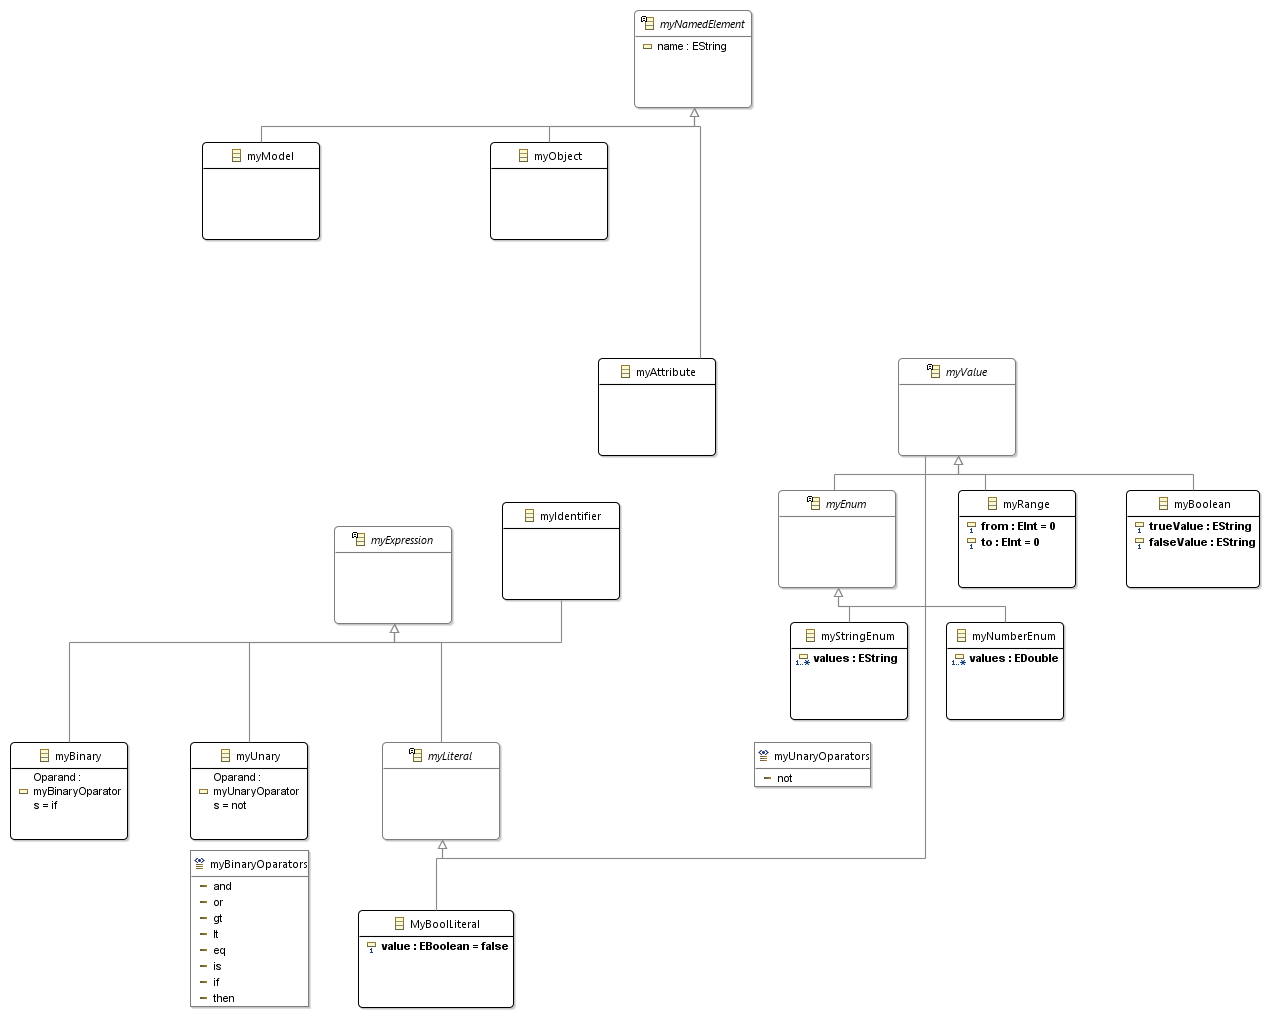
\includegraphics[scale=0.7]{pictures/taxView.png}
\caption{Taxonomy View}
\end{figure}


\section{The Meta-model}
\begin{figure}[ht!]
\centering
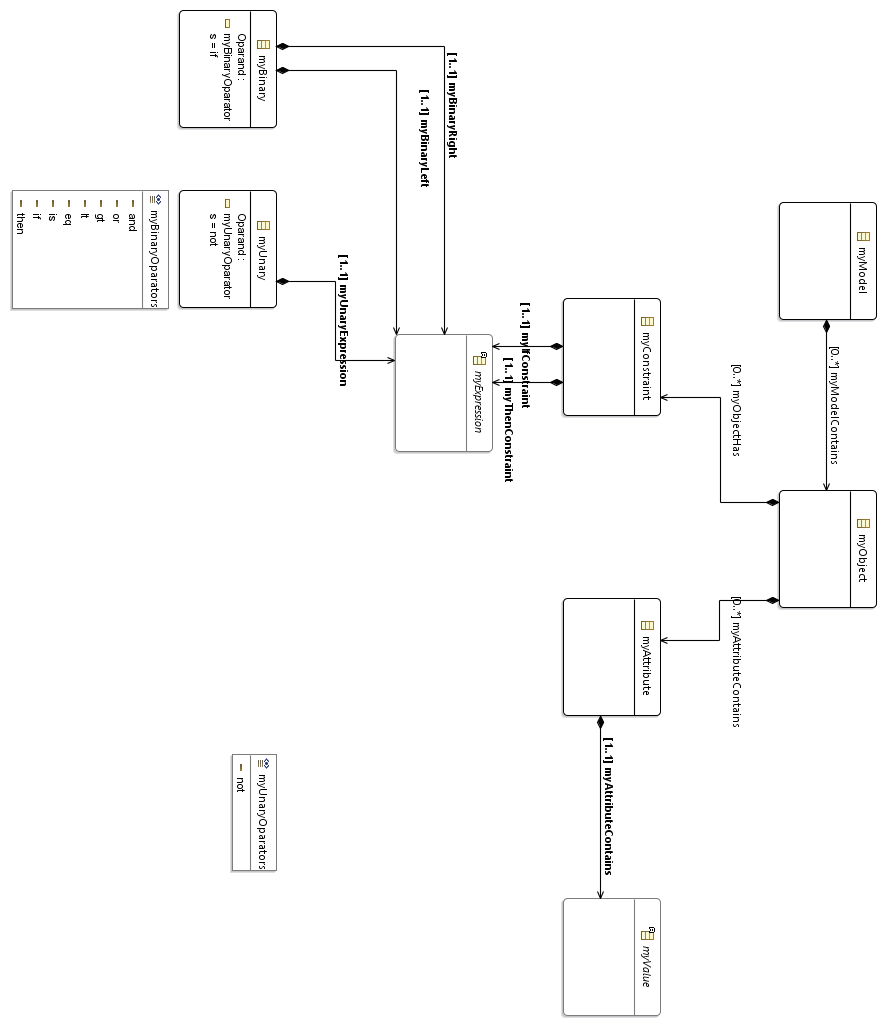
\includegraphics[scale=0.7]{pictures/partView.png}
\caption{Partonomy View}
\end{figure}

\begin{figure}[ht!]
\centering
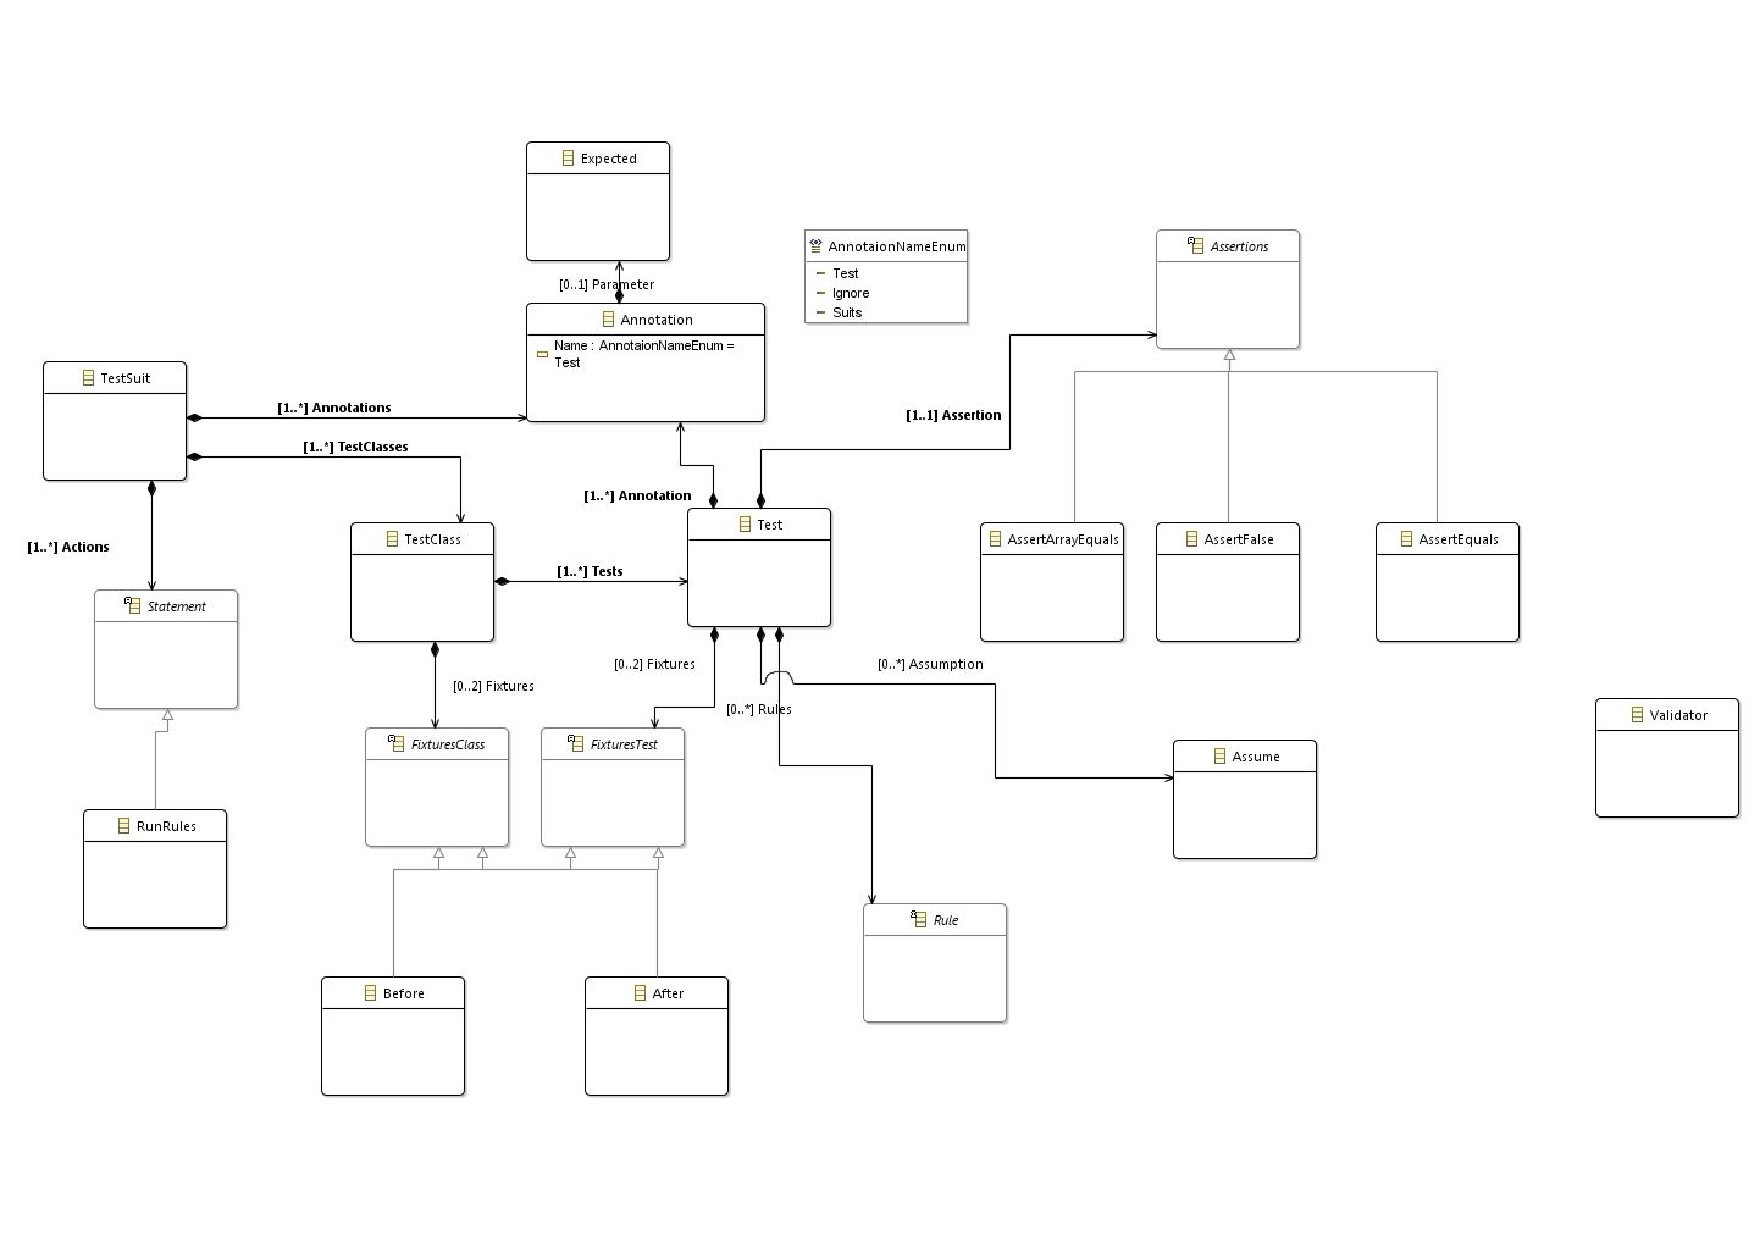
\includegraphics[scale=0.7]{pictures/mrha.pdf}
\caption{meta model}
\end{figure}

% 4. Static semantics (constraints, type system). If you have a type checker describe brieflyhow it works and present the key rules (functions). If you have constraints, includethe entire implementation of the constraints in Xtend with comments explaining the intended semantics in English. No further description is needed.
\section{Static semantics}

% 5. Xtext grammar of your language (Concrete Syntax). Just include the .xtext file. You can omit the top imports and other boiler plate, but we want to see all productions. No commentary is expected.
\section{Xtext grammar of your language}
\java{../configproject/xtext/org.xtext.example.smdpdsl/src/org/xtext/example/mydsl/SmdpDsl.xtext}{static}

% 6. Descriptions of back-ends: the most relevant fragments of your back ends implementation with commentary (max 5 pages in total for both back-ends, not 10 pages). Describe briefly the architecture selected for the two backends (perhaps present an architectural diagram), and show the key aspects of implementation of both back-ends.
\section{Description of back-ends}
\subsection{Back-end |}
\subsection{Back-end ||}

% 7. Test methods and artefacts: Hand in max 1 page description of your test strategy (half a page is recommended) plus max 3 pages of examples of test cases. All in a single PDF file
\section{Test methods and artefacts}
The tests for this project, have been split in three files: SmdpDslParserTest.xtend, SmdpDslGeneratorTest.xtend and SmdpDslValidator.xtend.\\
The tests for the parser tests how the types from the concrete syntax is inferred from the model and how the parser behaves when given an unexpected input, like a instance of a model which contains two strings in the name instead of one. The tests are created to test input of size zero, one and many, which means that most tests are represented in three cases.\\
The focus of the tests made in SmdpDslValidator have been to test how well  



All tests have been created towards the end of the project, which isn't optimal in terms of being able to use the tests and results from the tests. Some of the tests have shown that some errors exists in the project. One example of this is the testMyObjectsWithEmptyAttributesList method in SmdpDslParserTest. In this test no attributes have provided, but the size of attributes is one, but should have been zero.\\
If this test was made at an earlier stage of the project, it would have been possible to resolve this error. But due to time constraint at the time of writing the tests, the error, and others found in different tests, are still present.\\
Even though some of the tests have demonstrated unexpected outputs, we believe that these can be catogorized as minor errors without a critical impact on the system. 
%-------- END --------------------------------------------------------------------------------
\end{document}